%! suppress = LineBreak
\section{Идея генератора оружия}

Исходный код доступен в репозитории\cite{s7}.

\subsection{Общая идея}

Генерируемое оружие основано на системах частиц из программ NEAT Projectiles и
NEAT Particles\cite{s2}\cite{s3}. Каждое оружие содержит в себе нейронную сеть (Рисунок~\ref{Weapon}). Каждый кадр анимации каждая частица, выпущенная из оружия, подает на вход в нейронную сеть свое текущее положение относительно точки выстрела {\small \textbf{(RelativePos.x, RelativePos.y)}} и расстояние от точки выстрела {\small \textbf{DistanceFromOrigin}}. После этого нейронная сеть активируется и выводит единичный вектор силы {\small \textbf{(x, y)}}, которая приложена к частице, её компоненту {\small \textbf{hue}} цветовой модели HSV, её максимальную скорость {\small \textbf{maxSpeed}} и длину вектора силы {\small \textbf{force}} для этого анимационного кадра.

\begin{figure}[ht]
    \begin{center}
        \scalebox{0.18}{
            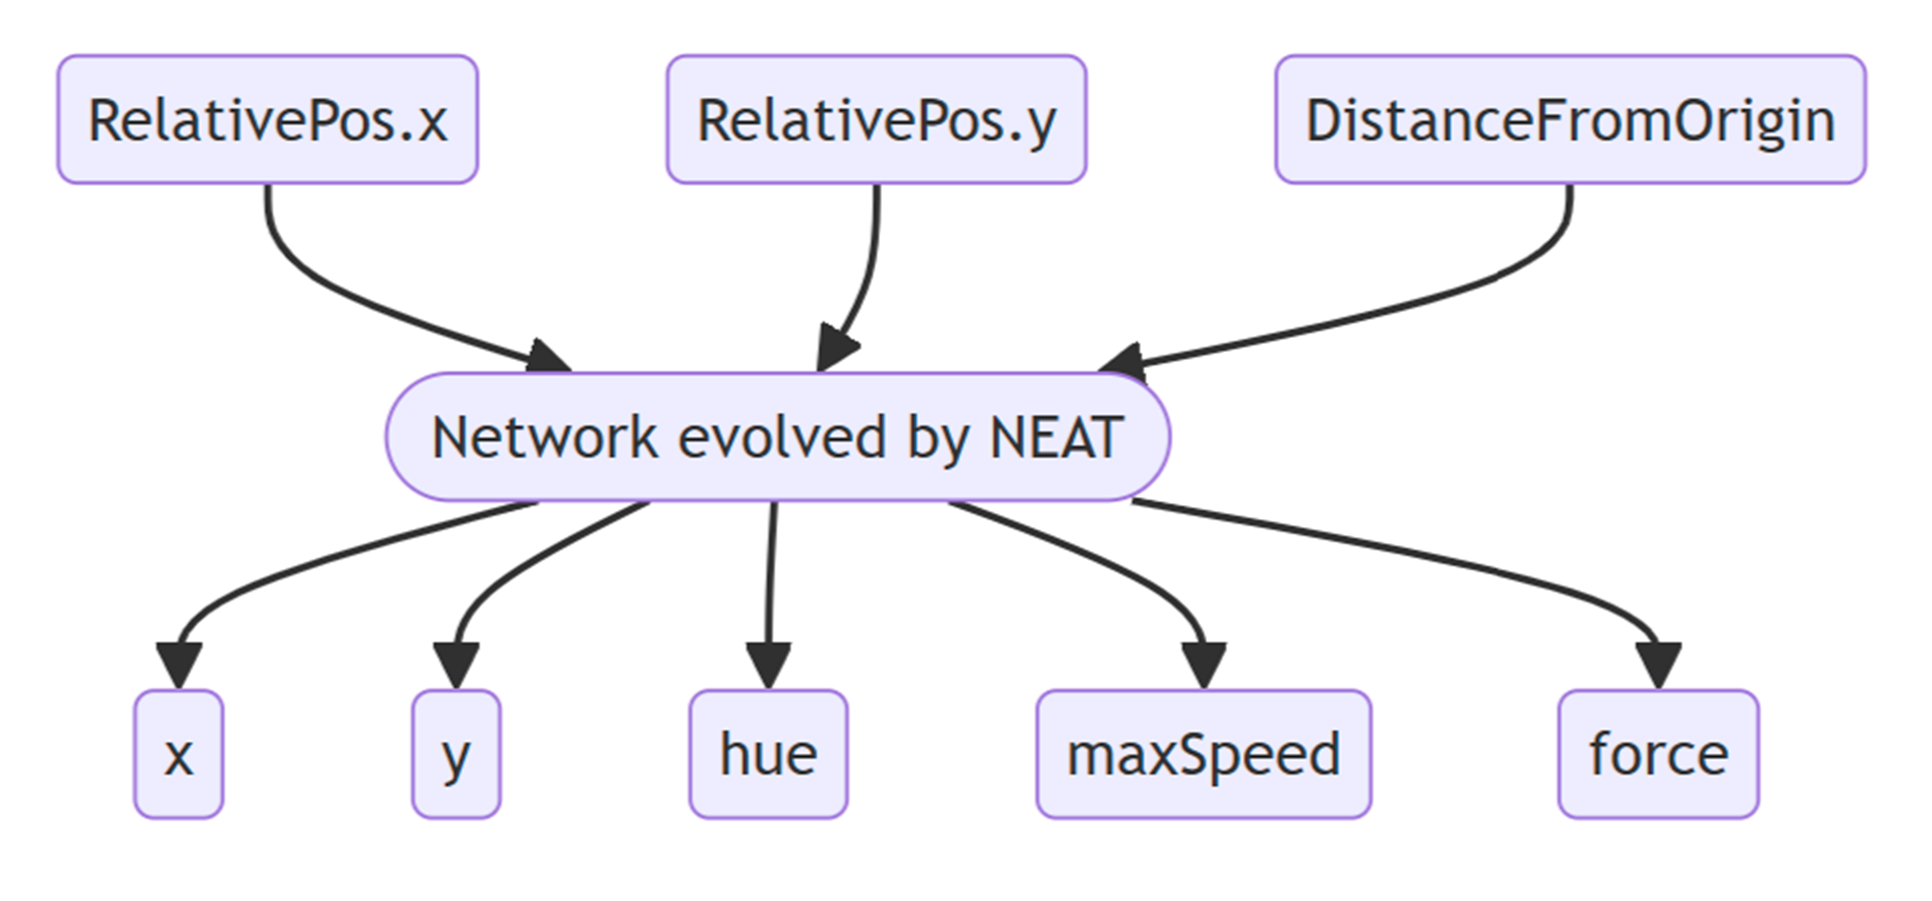
\includegraphics{images/GenIdea}
        }

        \caption{
            \label{Weapon}
            Как нейронная сеть управляет снарядами.}
    \end {center}
\end {figure}

Поскольку оружие представляется нейронной сетью, можно генерировать новое оружие, изменяя веса и топологию нейронной сети. Для этой цели был выбран алгоритм NEAT\cite{s1}, который расшифровывается как нейроэволюция расширяющихся топологий (NeuroEvolution of Augmenting Topologies). Это метод, предназначенный для эволюции искусственных нейронных сетей с помощью генетического алгоритма. Главная идея NEAT заключается в том, что эволюцию наиболее эффективно начинать с маленьких, простых сетей, которые постепенно становятся всё более сложными с каждым поколением.

